\documentclass[11pt,a4paper]{article}
\usepackage{amsmath}\usepackage{amssymb}\usepackage[table]{xcolor}
\usepackage{tabularx}\usepackage{multirow}\usepackage{geometry}
\usepackage{enumitem}\usepackage{parskip}\usepackage{titlesec}
\usepackage{tocloft}\usepackage[most]{tcolorbox}
\usepackage{tikz}\usepackage{pgfplots}\pgfplotsset{compat=1.18}\usetikzlibrary{arrows.meta,calc,positioning,shapes.geometric,patterns}
\geometry{margin=2.5cm}
\titleformat{\section}{\large\bfseries}{}{0em}{}
\setlength{\cftbeforesecskip}{6pt}
\definecolor{q1color}{HTML}{D6EAF8}\definecolor{q2color}{HTML}{D5F5E3}
\definecolor{q3color}{HTML}{FDEBD0}\definecolor{q4color}{HTML}{F9E79F}
\definecolor{q5color}{HTML}{E8DAEF}\definecolor{q6color}{HTML}{FADBD8}
\definecolor{q7color}{HTML}{D1F2EB}\definecolor{q8color}{HTML}{FCF3CF}
\definecolor{q9color}{HTML}{EBDEF0}\definecolor{q10color}{HTML}{F5EEF8}
\newenvironment{mstab}[1]{%
  {\color{#1!75!black}\nobreak Mark Scheme}\par\nopagebreak\smallskip
  \arrayrulecolor{#1!70!black}\renewcommand{\arraystretch}{1.3}%
  \tabularx{\textwidth}{|>{\columncolor{#1!12}\raggedright\arraybackslash}p{1.9cm}|>{\columncolor{#1!12}}X|>{\columncolor{#1!12}\centering\arraybackslash}p{1.1cm}|}%
  \hline\rowcolor{#1!45} Question & Answer & Marks \\ \hline}{%
  \endtabularx\arrayrulecolor{black}\par\medskip}
\newtcolorbox{ansbox}[1]{colback=#1!8,colbacktitle=#1!30,colframe=#1!70!black,coltitle=black,fonttitle=\normalfont,title=Worked Solution,boxrule=0.6pt,arc=2mm,left=4pt,right=4pt,top=4pt,bottom=4pt,breakable}
\newcommand{\topiclabel}[1]{\hfill\normalfont\small\itshape\textcolor{black!55}{#1}}
\newcommand{\examq}[4]{\section[#1 - Q#2]{#1 - Q#2 - #3 - #4}}
\begin{document}
\begin{center}
  {\LARGE \textbf{Cambridge O Level Additional Mathematics 4037/21/M/J/16}}\\[6pt]
  {\large May/June 2016 -- Mark Scheme \& Worked Solutions}
\end{center}
\bigskip

% ===================================================== Q1
\examq{4037/21/M/J/16}{1}{Quadratic Functions}{3}
\begin{mstab}{q1color}
 & $x^2-2x-15\ [>0]$ \newline \textit{expands and rearranges to a 3 term quadratic} & M1 \\ \hline
 & critical values $-3$ and $5$ \newline \textit{not from wrong working} & A1 \\ \hline
\multirow{-3}{1.9cm}{1} & $x<-3$, \ $x>5$ \newline \textit{mark final inequality; A0 if spurious attempt to combine, e.g.\ $5<x<-3$} & A1 \\ \hline
\end{mstab}
\begin{ansbox}{q1color}
\[ (x-4)(x+2)>7 \;\Rightarrow\; x^2-2x-8>7 \;\Rightarrow\; x^2-2x-15>0 \]
\[ (x-5)(x+3)>0 \;\Rightarrow\; \text{critical values } x=-3,\ x=5 \]
The quadratic is positive outside its roots:
\[ \boxed{x<-3 \quad\text{or}\quad x>5} \]
\end{ansbox}

% ===================================================== Q2
\examq{4037/21/M/J/16}{2}{Excluded from the present curriculum}{4}
\begin{mstab}{q2color}
2(a) & Correct Venn diagram: $A$ inside $B$ inside $C$ (nested circles) & B1 \\ \hline
2(b)(i) & $h\in P$ \newline \textit{Allow $\{m,a,t,h,s\}$ for $P$} & B1 \\ \hline
2(b)(ii) & $n(P\cap Q)=2$ & B1 \\ \hline
2(b)(iii) & $\{t,\ h,\ s\}$ & B1 \\ \hline
\end{mstab}
\begin{ansbox}{q2color}
\textbf{(a)} $A\subset B$ and $B\subset C$: draw $A$ entirely inside $B$, and $B$ entirely inside $C$.
\begin{center}
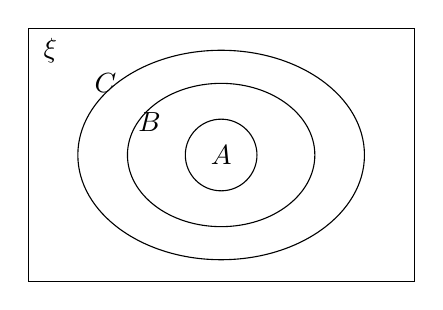
\begin{tikzpicture}[scale=0.7]
\draw (0,0) rectangle (7,4.6); \node at (0.4,4.2) {$\xi$};
\draw (3.5,2.3) ellipse (2.6 and 1.9); \node at (1.4,3.6) {$C$};
\draw (3.5,2.3) ellipse (1.7 and 1.3); \node at (2.2,2.9) {$B$};
\draw (3.5,2.3) circle (0.65); \node at (3.5,2.3) {$A$};
\end{tikzpicture}
\end{center}

\textbf{(b)} $P=\{m,a,t,h,s\}$, \ $Q=\{e,x,a,m\}$.

\textbf{(i)} \ $\boxed{h\in P}$

\textbf{(ii)} The common letters are $m$ and $a$: \ $\boxed{n(P\cap Q)=2}$

\textbf{(iii)} Letters of \emph{maths} not in \emph{exam}:
\[ P\cap Q'=\boxed{\{t,\ h,\ s\}} \]
\end{ansbox}

% ===================================================== Q3
\examq{4037/21/M/J/16}{3}{Logarithmic \& Exponential Functions}{6}
\begin{mstab}{q3color}
3(i) & $-2$ & B1 \\ \hline
3(ii) & $-n$ & B1 \\ \hline
 & $\lg 20-\lg 4=\lg 5$ or $\log_5 10=\dfrac{1}{\lg 5}$ \newline \textit{One log law only used correctly} & M1 \\ \hline
\multirow{-2}{1.9cm}{3(iii)} & $(\lg 5)^2$, \ $y=5$ \newline \textit{answer only does not score} & A1 \\ \hline
 & $6x^2=600$ \newline \textit{Condone missing base} & B1 \\ \hline
\multirow{-2}{1.9cm}{3(iv)} & $x=10$ only & B1 \\ \hline
\end{mstab}
\begin{ansbox}{q3color}
\textbf{(i)}
\[ \log_\pi\left(\frac{1}{\pi^2}\right)=\log_\pi\pi^{-2}=\boxed{-2} \]

\textbf{(ii)}
\[ \lg\left(\frac{1}{10^n}\right)=\lg 10^{-n}=\boxed{-n} \]

\textbf{(iii)}
\[ \lg 20-\lg 4=\lg\frac{20}{4}=\lg 5, \qquad \log_5 10=\frac{\lg 10}{\lg 5}=\frac{1}{\lg 5} \]
\[ \frac{\lg 20-\lg 4}{\log_5 10}=\frac{\lg 5}{\;\frac{1}{\lg 5}\;}=(\lg 5)^2 \;\Rightarrow\; \boxed{y=5} \]

\textbf{(iv)}
\[ \log_\pi 2x+\log_\pi 3x=\log_\pi 600 \;\Rightarrow\; \log_\pi(6x^2)=\log_\pi 600 \;\Rightarrow\; 6x^2=600 \]
\[ x^2=100 \;\Rightarrow\; x=\pm10 \]
$x=-10$ is rejected since $\log_\pi 2x$ requires $x>0$:
\[ \boxed{x=10} \]
\end{ansbox}

% ===================================================== Q4
\examq{4037/21/M/J/16}{4}{Circular Measure}{5}
\begin{mstab}{q4color}
4(i) & $\dfrac{\pi}{3}$ isw & B1 \\ \hline
 & [Area triangle $ABC=$] $\dfrac{1}{2}\times10^2\sin\left(\text{their }\dfrac{\pi}{3}\right)$ oe \newline \textit{seen or implied by $25\sqrt{3}$ or $43.3(0\ldots)$} & M1 \\ \hline
 & [Area 1 sector $=$] $\dfrac{1}{2}\times5^2\times\text{their }\dfrac{\pi}{3}$ oe or $\dfrac{\text{their }60^\circ}{360}\times\pi\times5^2$ \newline \textit{seen or implied by $\dfrac{25\pi}{6}$ or $13.0(8\ldots)$ or $13.09$} & M1 \\ \hline
 & Complete correct plan \newline \textit{e.g.\ their triangle $-$ 3(their sector)} & M1 \\ \hline
\multirow{-4}{1.9cm}{4(ii)} & $4.03(1\ldots)$ or $25\sqrt{3}-\dfrac{25\pi}{2}$ isw \newline \textit{Units not required} & A1 \\ \hline
\end{mstab}
\begin{ansbox}{q4color}
\textbf{(i)} Each side of triangle $ABC$ is $5+5=10$ cm, so the triangle is equilateral:
\[ \boxed{\theta=\frac{\pi}{3}} \]

\textbf{(ii)}
\[ \text{Area of triangle }ABC=\frac{1}{2}\times10\times10\times\sin\frac{\pi}{3}=25\sqrt{3}=43.301\ldots \]
\[ \text{Area of one sector}=\frac{1}{2}\times5^2\times\frac{\pi}{3}=\frac{25\pi}{6}=13.089\ldots \]
\[ \text{Shaded area}=25\sqrt{3}-3\times\frac{25\pi}{6}=25\sqrt{3}-\frac{25\pi}{2} \]
\[ \boxed{\text{Shaded area}=4.03\ \mathrm{cm^2}} \]
\end{ansbox}

% ===================================================== Q5
\examq{4037/21/M/J/16}{5}{Indices \& Surds}{6}
\begin{mstab}{q5color}
 & $\dfrac{\sqrt{8}\left(\sqrt{7}+\sqrt{5}\right)}{\left(\sqrt{7}-\sqrt{5}\right)\left(\sqrt{7}+\sqrt{5}\right)}$ and attempt to multiply & M1 \\ \hline
 & $\dfrac{\sqrt{56}+\sqrt{40}}{2}$ oe \newline \textit{not from wrong working} & A1 \\ \hline
\multirow{-3}{1.9cm}{5(a)} & $\sqrt{14}+\sqrt{10}$ & A1 \\ \hline
 & $q^2+4\sqrt{3}\,q+12$ soi & B1 \\ \hline
 & $28=q^2+12$ oe \newline \textit{can be implied by 4 and 16 or $-4$ and $-16$} & M1 \\ \hline
\multirow{-3}{1.9cm}{5(b)} & $q=4,\ -4$ \quad $p=16,\ -16$ \newline \textit{all values} & A1 \\ \hline
\end{mstab}
\begin{ansbox}{q5color}
\textbf{(a)} Multiply numerator and denominator by $\sqrt{7}+\sqrt{5}$:
\[ \frac{\sqrt{8}}{\sqrt{7}-\sqrt{5}}=\frac{\sqrt{8}\left(\sqrt{7}+\sqrt{5}\right)}{\left(\sqrt{7}-\sqrt{5}\right)\left(\sqrt{7}+\sqrt{5}\right)}=\frac{\sqrt{56}+\sqrt{40}}{7-5} \]
\[ =\frac{2\sqrt{14}+2\sqrt{10}}{2}=\boxed{\sqrt{14}+\sqrt{10}} \]

\textbf{(b)}
\[ \left(q+2\sqrt{3}\right)^2=q^2+4\sqrt{3}\,q+12 \]
Comparing with $28+p\sqrt{3}$:
\[ \text{rational parts: } q^2+12=28 \;\Rightarrow\; q^2=16 \;\Rightarrow\; q=\pm4 \]
\[ \text{surd parts: } p=4q \]
\[ \boxed{q=4,\ p=16 \quad\text{or}\quad q=-4,\ p=-16} \]
\end{ansbox}

% ===================================================== Q6
\examq{4037/21/M/J/16}{6}{Quadratic Functions \textperiodcentered\ Equations, Inequalities \& Graphs}{8}
\begin{mstab}{q6color}
6(i) & $4(x+1)^2-9$ \newline \textit{one mark for each of $p$, $q$, $r$ correct in a correctly formatted expression; allow correct equivalent values; \newline If B0 then SC2 for $4(x+1)-9$ or SC1 for correct 3 values seen in incorrect format e.g.\ $4(x+x1)-9$ or $(4x+1)^2-9$ or for a correct completed square form of the original expression in a different but correct format, e.g.\ $(2x+2)^2-9$} & B3,2, 1,0 \\ \hline
6(ii) & $(-1,\ 9)$ \newline \textit{B1FT $(-q,\ -r)$, $r<0$, for each correct coordinate} & B2FT \\ \hline
 & Correct symmetric W shape with cusps on $x$-axis & B1 \\ \hline
 & $y$-intercept marked at 5 only or coords indicated on graph & B1 \\ \hline
\multirow{-3}{1.9cm}{6(iii)} & $x$-intercepts marked at $-2.5$ and $0.5$ only on $x$-axis or coords indicated on graph or close by & B1 \\ \hline
\end{mstab}
\begin{ansbox}{q6color}
\textbf{(i)}
\[ 4x^2+8x-5=4\left(x^2+2x\right)-5=4\left[(x+1)^2-1\right]-5 \]
\[ \boxed{4x^2+8x-5=4(x+1)^2-9}\qquad(p=4,\ q=1,\ r=-9) \]

\textbf{(ii)} The vertex of $y=4x^2+8x-5$ is $(-1,\ -9)$; the modulus reflects it in the $x$-axis:
\[ \boxed{(-1,\ 9)} \]

\textbf{(iii)} $4x^2+8x-5=(2x+5)(2x-1)=0 \Rightarrow x=-2.5,\ 0.5$; \ at $x=0$, $y=|-5|=5$.
\begin{center}
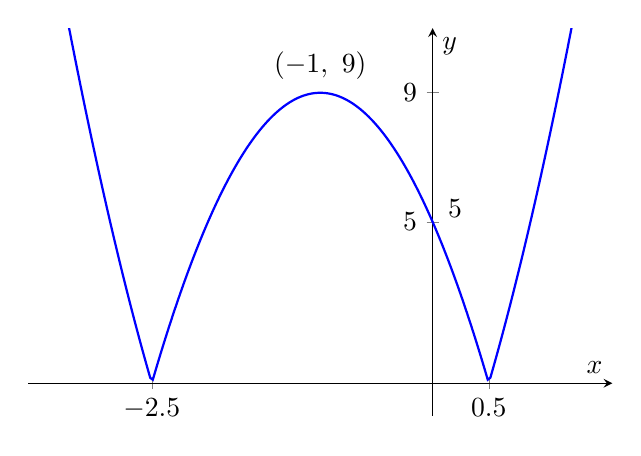
\begin{tikzpicture}
\begin{axis}[width=9cm,height=6.5cm,axis lines=middle,xmin=-3.6,xmax=1.6,ymin=-1,ymax=11,xlabel={$x$},ylabel={$y$},xtick={-2.5,0.5},xticklabels={$-2.5$,$0.5$},ytick={5,9},samples=200]
\addplot[thick,blue,domain=-3.3:1.3] {abs(4*x^2+8*x-5)};
\node[anchor=west] at (axis cs:0.05,5.4) {$5$};
\node[anchor=south] at (axis cs:-1,9.1) {$(-1,\ 9)$};
\end{axis}
\end{tikzpicture}
\end{center}
A W shape with cusps on the $x$-axis at $(-2.5,\ 0)$ and $(0.5,\ 0)$, crossing the $y$-axis at $(0,\ 5)$.
\end{ansbox}

% ===================================================== Q7
\examq{4037/21/M/J/16}{7}{Vectors in Two Dimensions}{7}
\begin{mstab}{q7color}
7(i)(a) & $\mathbf{q}-\mathbf{p}$ & B1 \\ \hline
7(i)(b) & $2\mathbf{q}-2\mathbf{p}$ or $2(\mathbf{q}-\mathbf{p})$ & B1 \\ \hline
 & The points are collinear oe & B1 \\ \hline
\multirow{-2}{1.9cm}{7(ii)} & $\overrightarrow{PQ}$ is a (scalar) multiple of $\overrightarrow{QR}$ and they have a point in common oe \newline \textit{Condone $\overrightarrow{PQ}$ is parallel to $\overrightarrow{QR}$ and \ldots} & B1 \\ \hline
 & [$\overrightarrow{OR}=$] $4\mathbf{i}-3\mathbf{j}$ oe soi & B1 \\ \hline
 & $\sqrt{4^2+(-3)^2}\ (=5)$ \newline \textit{condone $\sqrt{4^2+3^2}$; may be implied by correct answer or correct FT answer} & M1 \\ \hline
\multirow{-3}{1.9cm}{7(iii)} & $\dfrac{1}{5}(4\mathbf{i}-3\mathbf{j})$ oe & A1 \\ \hline
\end{mstab}
\begin{ansbox}{q7color}
\textbf{(i)(a)}
\[ \overrightarrow{PQ}=\overrightarrow{OQ}-\overrightarrow{OP}=\boxed{\mathbf{q}-\mathbf{p}} \]
\textbf{(b)}
\[ \overrightarrow{QR}=\overrightarrow{OR}-\overrightarrow{OQ}=(3\mathbf{q}-2\mathbf{p})-\mathbf{q}=\boxed{2\mathbf{q}-2\mathbf{p}=2(\mathbf{q}-\mathbf{p})} \]

\textbf{(ii)} $\overrightarrow{QR}=2\overrightarrow{PQ}$, so $PQ$ and $QR$ are parallel, and they share the point $Q$. Hence \textbf{$P$, $Q$ and $R$ are collinear}.

\textbf{(iii)}
\[ \overrightarrow{OR}=3(2\mathbf{i}+\mathbf{j})-2(\mathbf{i}+3\mathbf{j})=6\mathbf{i}+3\mathbf{j}-2\mathbf{i}-6\mathbf{j}=4\mathbf{i}-3\mathbf{j} \]
\[ \left|\overrightarrow{OR}\right|=\sqrt{4^2+(-3)^2}=5 \]
\[ \text{Unit vector}=\boxed{\frac{1}{5}(4\mathbf{i}-3\mathbf{j})} \]
\end{ansbox}

% ===================================================== Q8
\examq{4037/21/M/J/16}{8}{Binomial Theorem}{7}
\begin{mstab}{q8color}
8(a)(i) & $a^4+4a^3b+6a^2b^2+4ab^3+b^4$ final answer \newline \textit{$-1$ each error/omission} & B2,1,0 \\ \hline
 & $6\left(\dfrac{2x}{5}\right)^2\left(\dfrac{1}{x}\right)^2$ soi \newline \textit{Could be in full expansion} & M1 \\ \hline
\multirow{-2}{1.9cm}{8(a)(ii)} & $\dfrac{24}{25}$ or $0.96$ isw \newline \textit{Must be explicitly identified} & A1 \\ \hline
 & $\dfrac{n(n-1)(n-2)}{6}\left(\dfrac{1}{8}\right)=\dfrac{5n}{12}$ soi leading to a cubic or quadratic $\left(n^2-3n-18=0\right)$ \newline \textit{Must attempt to expand and remove fractions} & M1 \\ \hline
 & Solves their quadratic $[(n-6)(n+3)]$ \newline \textit{must have come from a valid attempt} & M1 \\ \hline
\multirow{-3}{1.9cm}{8(b)} & $[n=]\ 6$ only, not from wrong working \newline \textit{Must be $n$ if labelled} & A1 \\ \hline
\end{mstab}
\begin{ansbox}{q8color}
\textbf{(a)(i)}
\[ (a+b)^4=a^4+\binom{4}{1}a^3b+\binom{4}{2}a^2b^2+\binom{4}{3}ab^3+b^4 \]
\[ \boxed{(a+b)^4=a^4+4a^3b+6a^2b^2+4ab^3+b^4} \]

\textbf{(ii)} Put $a=\dfrac{2x}{5}$, $b=\dfrac{1}{x}$. The term independent of $x$ is the $6a^2b^2$ term:
\[ 6\left(\frac{2x}{5}\right)^2\left(\frac{1}{x}\right)^2=6\times\frac{4x^2}{25}\times\frac{1}{x^2}=\boxed{\frac{24}{25}} \]

\textbf{(b)} Coefficient of $x^3$ in $\left(1+\dfrac{x}{2}\right)^n$:
\[ \binom{n}{3}\left(\frac{1}{2}\right)^3=\frac{n(n-1)(n-2)}{6}\times\frac{1}{8}=\frac{5n}{12} \]
Divide by $n$ ($n\neq0$) and multiply by 48:
\[ (n-1)(n-2)=20 \;\Rightarrow\; n^2-3n-18=0 \;\Rightarrow\; (n-6)(n+3)=0 \]
$n$ is a positive integer, so
\[ \boxed{n=6} \]
\end{ansbox}

% ===================================================== Q9
\examq{4037/21/M/J/16}{9}{Trigonometry}{8}
\begin{mstab}{q9color}
9(a) & $a=2$ \quad $b=4$ \quad $c=-2$ \newline \textit{B1 for each correct value} & B3 \\ \hline
9(b)(i) & sinusoidal curve \newline symmetrical about $y$-axis \newline clear intent to have amplitude of 2 \newline 2 cycles \newline \textit{If not fully correct max B2} & B3,2, 1,0 \\ \hline
9(b)(ii) & $-\dfrac{\pi}{2}$, \ $-\dfrac{\pi}{6}$, \ $\dfrac{\pi}{6}$, \ $\dfrac{\pi}{2}$, \ $-\dfrac{\pi}{3}$, \ $\dfrac{\pi}{3}$ cao \newline \textit{B1 for any 4 correct} & B2 \\ \hline
\end{mstab}
\begin{ansbox}{q9color}
\textbf{(a)} $y=a\tan bx+c$. The period of $\tan bx$ is $\dfrac{\pi}{b}=\dfrac{\pi}{4}$, so $b=4$.
\[ (0,\ -2):\quad -2=a\tan0+c \;\Rightarrow\; c=-2 \]
\[ \left(\frac{\pi}{16},\ 0\right):\quad 0=a\tan\frac{\pi}{4}-2=a-2 \;\Rightarrow\; a=2 \]
\[ \boxed{a=2,\quad b=4,\quad c=-2} \]

\textbf{(b)(i)} $y=2\cos3x+1$: amplitude 2, period $\dfrac{2\pi}{3}$ (2 cycles in $-\dfrac{2\pi}{3}\leqslant x\leqslant\dfrac{2\pi}{3}$), maximum 3, minimum $-1$, symmetrical about the $y$-axis.
\begin{center}
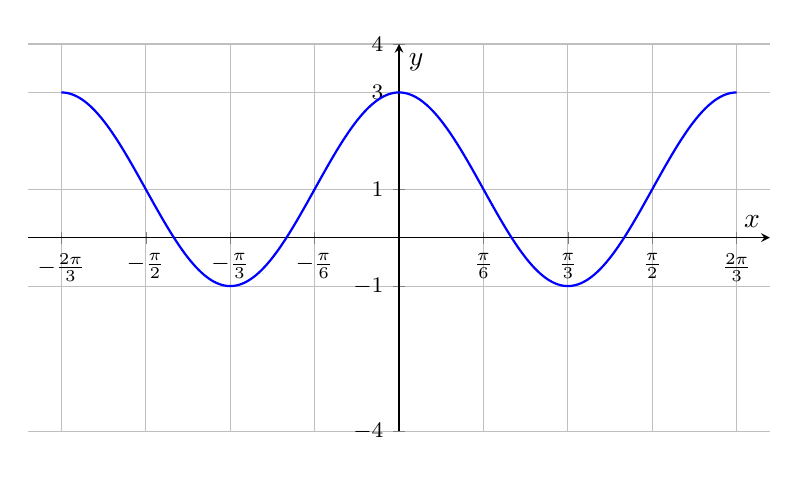
\begin{tikzpicture}
\begin{axis}[width=11cm,height=6.5cm,axis lines=middle,xmin=-2.3,xmax=2.3,ymin=-4,ymax=4,xlabel={$x$},ylabel={$y$},
xtick={-2.0944,-1.5708,-1.0472,-0.5236,0.5236,1.0472,1.5708,2.0944},
xticklabels={$-\frac{2\pi}{3}$,$-\frac{\pi}{2}$,$-\frac{\pi}{3}$,$-\frac{\pi}{6}$,$\frac{\pi}{6}$,$\frac{\pi}{3}$,$\frac{\pi}{2}$,$\frac{2\pi}{3}$},
ytick={-4,-1,1,3,4},grid=major,samples=300,ticklabel style={font=\footnotesize}]
\addplot[thick,blue,domain=-2.0944:2.0944] {2*cos(deg(3*x))+1};
\end{axis}
\end{tikzpicture}
\end{center}

\textbf{(ii)} $(2\cos3x+1)^2=1 \Rightarrow 2\cos3x+1=1$ or $2\cos3x+1=-1$, i.e.\ where the graph meets $y=1$ or $y=-1$.
\[ 2\cos3x+1=1:\quad \cos3x=0 \;\Rightarrow\; 3x=\pm\frac{\pi}{2},\ \pm\frac{3\pi}{2} \;\Rightarrow\; x=\pm\frac{\pi}{6},\ \pm\frac{\pi}{2} \]
\[ 2\cos3x+1=-1:\quad \cos3x=-1 \;\Rightarrow\; 3x=\pm\pi \;\Rightarrow\; x=\pm\frac{\pi}{3} \]
\[ \boxed{x=-\frac{\pi}{2},\ -\frac{\pi}{3},\ -\frac{\pi}{6},\ \frac{\pi}{6},\ \frac{\pi}{3},\ \frac{\pi}{2}} \]
\end{ansbox}

% ===================================================== Q10
\examq{4037/21/M/J/16}{10}{Permutations \& Combinations}{8}
\begin{mstab}{q10color}
 & $2\times4!$ or $\dfrac{2\times5!}{5}$ oe & M1 \\ \hline
\multirow{-2}{1.9cm}{10(a)(i)} & $48$ & A1 \\ \hline
 & ${}^{5}\mathrm{P}_3$ or $\dfrac{5!}{2!}$ or $5\times4\times3$ oe & M1 \\ \hline
\multirow{-2}{1.9cm}{10(a)(ii)} & $60$ & A1 \\ \hline
 & $4\times2[!]\times3$ oe \newline \textit{Correct first step implied by a correct product of two elements} & M1 \\ \hline
\multirow{-2}{1.9cm}{10(b)(i)} & $24$ & A1 \\ \hline
 & $3!$ or $3\times3$ seen & M1 \\ \hline
\multirow{-2}{1.9cm}{10(b)(ii)} & $18$ & A1 \\ \hline
\end{mstab}
\begin{ansbox}{q10color}
\textbf{(a)(i)} The last digit must be 2 or 4 (2 ways); the other 4 digits fill the remaining places in $4!$ ways:
\[ 2\times4!=2\times24=\boxed{48} \]

\textbf{(ii)} Choose and arrange 3 of the 5 digits:
\[ {}^{5}\mathrm{P}_3=5\times4\times3=\boxed{60} \]

\textbf{(b)(i)} Treat the two women as a block occupying 2 adjacent chairs: 4 positions for the block, 2 ways to order the women, then 3 chairs remain for the man:
\[ 4\times2!\times3=\boxed{24} \]

\textbf{(ii)} The three people occupy 3 adjacent chairs: 3 possible positions for the block, and $3!$ ways to arrange the people within it:
\[ 3\times3!=3\times6=\boxed{18} \]
\end{ansbox}

% ===================================================== Q11
\examq{4037/21/M/J/16}{11}{Integration \textperiodcentered\ Straight-Line Graphs}{8}
\begin{mstab}{q1color}
11(i) & $\dfrac{3x^2}{2}-\dfrac{2x^{\frac{5}{2}}}{5}\ (+c)$ isw & B1+B1 \\ \hline
11(ii) & $(9,\ 0)$ oe \newline \textit{Not just $x=9$} & B1 \\ \hline
11(iii) & Substitute $(3,\ 9)$ into both lines \newline Or solves simultaneously ($6x=27-3x$ oe) to get $x=3$, $y=9$ \newline \textit{$3\times3=9$ and $\dfrac{27-3\times3}{2}=9$} & B1 \\ \hline
 & [Area $AOB=$] $\dfrac{1}{2}\times9\times9$ oe $\left(\dfrac{81}{2}\text{ or }40.5\right)$ \newline \textit{Uses their (ii). May split into 2 triangles (13.5 and 27). May integrate. Must be a complete method.} & M1 \\ \hline
 & $\left[\dfrac{3x^2}{2}-\dfrac{2x^{\frac{5}{2}}}{5}\right]$: their $\left(\dfrac{3(9)^2}{2}-\dfrac{2(9)^{\frac{5}{2}}}{5}\right)-0$ $(=24.3)$ \newline \textit{lower limit may be omitted but must be correct if seen} & M1 \\ \hline
 & their $\dfrac{81}{2}-$ their $\dfrac{243}{10}$ \newline \textit{must be from genuine attempts at area of triangle and area under curve} & M1 \\ \hline
\multirow{-4}{1.9cm}{11(iv)} & $16.2$ & A1 \\ \hline
\end{mstab}
\begin{ansbox}{q1color}
\textbf{(i)}
\[ \int\left(3x-x^{\frac{3}{2}}\right)\mathrm{d}x=\boxed{\frac{3x^2}{2}-\frac{2x^{\frac{5}{2}}}{5}+c} \]

\textbf{(ii)} On the $x$-axis, $y=0$ in $2y=27-3x$: \ $x=9$.
\[ \boxed{A(9,\ 0)} \]
(Check on the curve: $3(9)-9^{\frac{3}{2}}=27-27=0$.)

\textbf{(iii)} Substitute $(3,\ 9)$ into both lines:
\[ y=3x:\quad 3\times3=9 \;\checkmark \qquad\quad 2y=27-3x:\quad y=\frac{27-3\times3}{2}=\frac{18}{2}=9 \;\checkmark \]
So $B$ is $(3,\ 9)$.

\textbf{(iv)} The shaded region is triangle $OAB$ minus the area under the curve from $O$ to $A$.
\[ \text{Area of triangle }OAB=\frac{1}{2}\times9\times9=\frac{81}{2}=40.5 \]
\[ \int_0^9\left(3x-x^{\frac{3}{2}}\right)\mathrm{d}x=\left[\frac{3x^2}{2}-\frac{2x^{\frac{5}{2}}}{5}\right]_0^9=\frac{243}{2}-\frac{2(243)}{5}=121.5-97.2=24.3 \]
\[ \text{Shaded area}=40.5-24.3=\boxed{16.2} \]
\end{ansbox}

% ===================================================== Q12
\examq{4037/21/M/J/16}{12}{Differentiation}{10}
\begin{mstab}{q2color}
 & $\dfrac{\mathrm{d}y}{\mathrm{d}x}=\left[\dfrac{(x-1)(2)-(2x-5)}{(x-1)^2}\right]$ \newline \textit{Allow slips in $\dfrac{\mathrm{d}u}{\mathrm{d}x}$ and $\dfrac{\mathrm{d}v}{\mathrm{d}x}$ but must be explicit. Allow $(x-1)^2=x^2-2x+1$} & M1A1 \\ \hline
 & $-12$ isw & B1 \\ \hline
 & ALT using $y=\dfrac{-12x^2+14x-5}{x-1}$: \newline $-24x+14$ & B1 \\ \hline
\multirow{-4}{1.9cm}{12(i)} & $\dfrac{\mathrm{d}y}{\mathrm{d}x}=\left[\dfrac{(x-1)(-24x+14)-\left(-12x^2+14x-5\right)}{(x-1)^2}\right]$ \newline \textit{FT on their derivative of 3 term quadratic} & M1 A1FT \\ \hline
 & $\dfrac{\mathrm{d}^2y}{\mathrm{d}x^2}=k(x-1)^{-3}$ \newline \textit{No additional terms} & M1 \\ \hline
\multirow{-2}{1.9cm}{12(ii)} & $k=-6$ isw & A1 \\ \hline
 & their $\left(\dfrac{3}{(x-1)^2}-12\right)=0$ and find a value for $x$ \newline \textit{$12x^2-24x+9=0$ oe; \ $(2x-3)(2x-1)=0$ oe} & M1 \\ \hline
 & $x=0.5$ and $x=1.5$ & A1 \\ \hline
 & $y=2$ and $y=-22$ \newline \textit{if A0 A0 then A1 for a correct $(x,\ y)$ pair} & A1 \\ \hline
 & $\dfrac{-6}{(-0.5)^3}>0$ therefore min when $x=0.5$ oe \newline \textit{or $\dfrac{-6}{(-0.5)^3}=48$ therefore min when $x=0.5$ oe} & B1 \\ \hline
\multirow{-5}{1.9cm}{12(iii)} & $\dfrac{-6}{(0.5)^3}<0$ therefore max when $x=1.5$ oe \newline \textit{or $\dfrac{-6}{(0.5)^3}=-48$ therefore max when $x=1.5$ oe \newline M1A1 is possible from other methods} & B1 \\ \hline
\end{mstab}
\begin{ansbox}{q2color}
$y=\dfrac{2x-5}{x-1}-12x$.

\textbf{(i)} Quotient rule on the first term:
\[ \frac{\mathrm{d}y}{\mathrm{d}x}=\frac{(x-1)(2)-(2x-5)(1)}{(x-1)^2}-12=\frac{2x-2-2x+5}{(x-1)^2}-12 \]
\[ \boxed{\frac{\mathrm{d}y}{\mathrm{d}x}=\frac{3}{(x-1)^2}-12} \]

\textbf{(ii)} Write $\dfrac{\mathrm{d}y}{\mathrm{d}x}=3(x-1)^{-2}-12$:
\[ \frac{\mathrm{d}^2y}{\mathrm{d}x^2}=-6(x-1)^{-3} \;\Rightarrow\; \boxed{\frac{\mathrm{d}^2y}{\mathrm{d}x^2}=\frac{-6}{(x-1)^3}}\quad(k=-6) \]

\textbf{(iii)} Stationary points: $\dfrac{\mathrm{d}y}{\mathrm{d}x}=0$:
\[ \frac{3}{(x-1)^2}=12 \;\Rightarrow\; 12(x-1)^2=3 \;\Rightarrow\; 12x^2-24x+9=0 \;\Rightarrow\; 4x^2-8x+3=0 \]
\[ (2x-3)(2x-1)=0 \;\Rightarrow\; x=0.5 \ \text{or}\ x=1.5 \]
\[ x=0.5:\quad y=\frac{1-5}{-0.5}-6=8-6=2 \qquad\quad x=1.5:\quad y=\frac{3-5}{0.5}-18=-4-18=-22 \]
Nature:
\[ x=0.5:\quad \frac{\mathrm{d}^2y}{\mathrm{d}x^2}=\frac{-6}{(-0.5)^3}=48>0 \;\Rightarrow\; \text{minimum} \]
\[ x=1.5:\quad \frac{\mathrm{d}^2y}{\mathrm{d}x^2}=\frac{-6}{(0.5)^3}=-48<0 \;\Rightarrow\; \text{maximum} \]
\[ \boxed{(0.5,\ 2)\ \text{minimum};\qquad (1.5,\ -22)\ \text{maximum}} \]
\end{ansbox}

\end{document}
